\documentclass[12pt,a4wide]{article}

\usepackage{a4wide,amsmath,amssymb,graphicx,color}

\usepackage{listings,enumitem,calc,hyperref,caption,mmacells} 
\lstset{basicstyle=\small\ttfamily,breaklines=true,breakatwhitespace=true}

\definecolor{comment}{rgb}{0,0.3,0}
\lstset{language=Fortran}
\lstset{
  columns=flexible,
  basicstyle=\tt\footnotesize,
  keywordstyle=,
  identifierstyle=\color{black},
  commentstyle=\tt\color{comment},
  mathescape=false,
  escapebegin=\color{comment},
  showstringspaces=false,
  keepspaces=true
}

\title{H1jet, a fast program to compute transverse momentum distributions}


\begin{document}

\maketitle

\abstract{We present a fast code that computes the differential
  distribution of one of the final-state particles produced in a
  $2\to 2$ process.}

\section{Introduction}
\label{sec:intro}

\section{The method}
\label{sec:method}

We consider here a generic $2\to 2$ partonic process
$p_1 p_2 \to p_3 X$, where $p_1,p_2,p_3$ are partons, and $p_X$ is a
generic non-QCD particle $X$, e.g.\ a Higgs, of mass $m_X$. Our
program computes $d\sigma/dp_T$, where $p_T$ is the transverse
momentum of $p_X$ with respect to the beam axis, or the transverse
momentum of the recoiling jet originated by $p_3$. The possible
partonic subprocesses are $gg\to g X$, $q_f \bar q_{\bar f} \to g X$,
$q_f g\to q_f X$, $gq_f \to q_fX$, where $f,\bar f$ denotes quark (or
antiquark) flavours. The corresponding amplitudes $M_{ij}$ (with
$i,j=g,q_f$) are functions of the three Mandelstam invariants
\begin{equation}
  \label{eq:Mandelstam}
  \begin{split}
  \hat s & = (p_1+p_2)^2 = (p_3+p_X)^2 \,,\\
  \hat t & = (p_1-p_3)^2 = (p_2-p_X)^2 \,,\\
  \hat u & = (p_2-p_3)^2 = (p_1-p_X)^2 \,.
  \end{split}
\end{equation}
Without loss of generality, in the centre-of-mass frame of the
partonic collision, we can parametrise momenta as follows
\begin{equation}
  \label{eq:momenta}
  \begin{split}
  p_1&=\frac{\sqrt s}{2}(1,0,0,1)\,,\qquad p_3 = p_T(\cosh\eta,1,0,\sinh\eta)\,,\\
  p_2&=\frac{\sqrt s}{2}(1,0,0,1)\,,\qquad p_X = (\sqrt{m_X^2+p^2_T\cosh^2\eta},-1,0,-\sinh\eta)\,,
  \end{split}
\end{equation}
so that $\eta$ is in fact the rapidity of parton $p_3$ in the
centre-of-mass frame. The {\em partonic} $p_T$ spectrum for the
process initiated by partons $ij$ is given by
\begin{equation}
  \label{eq:partonic-pt}
  \frac{d\hat \sigma_{ij}}{dp_T} = \frac{p_T}{16\pi}\int d\eta \frac{M^2_{ij}(\hat s,\hat t,\hat u)}{E_X \hat s} \delta\left(\sqrt{\hat s} - p_T\cosh\eta-\sqrt{m_X^2+p^2_T\cosh^2\eta}\right)\,, 
\end{equation}
with $E_x=\sqrt{m_X^2+p^2_T\cosh^2\eta}$ the energy of the non-QCD
particle $p_X$.  The above equation selects two values of $\eta$, as
follows
\begin{equation}
\label{eq:eta-values}
  \eta = \ln(\hat x_M \pm \sqrt{\hat x_M^2-1})\,,\qquad \hat x_M\equiv\frac{\hat s-m_X^2}{2 p_T \sqrt{\hat s} }\,.
\end{equation}
The corresponding hadronic cross section reads, as usual
\begin{equation}
\label{eq:hadronic-pt}
  \frac{d\sigma}{dp_T} = \sum_{i,j} \int_0^1 dx_1\, f_{i/p}(x_1,\mu_F)\int_0^1 dx_2 \, f_{i/p}(x_1,\mu_F) \left[\frac{d\hat \sigma_{ij}}{dp_T} \Theta(s-\hat s) \Theta\left(\hat s-p_T-\sqrt{m_X^2+p^2_T}\right)  \right]_{\hat s=x_1x_2 s}\,.
\end{equation}
Since eq.~\eqref{eq:eta-values} give two monotonic functions of $\hat s$ for $s>p_T+\sqrt{m_X^2+p^2_T}$, varying $\hat s$ in the allowed range spans all possible values of $\eta$ in the range $-\eta_M<\eta<\eta_M$ with
\begin{equation}
\label{eq:eta-range}
\eta_M \equiv \ln(x_M + \sqrt{x_M^2-1})\,,\qquad  x_M\equiv\frac{s-m_X^2}{2 p_T \sqrt{s} }\,.
\end{equation}
This allows us to integrate over $\eta$ last, and obtain, after some
manipulations,
\begin{equation}
\label{eq:hadronic-pt-lumi}
  \frac{d\sigma}{dp_T} = \frac{p_T}{8 \pi}\int_{-\eta_M}^{\eta_M}\!d\eta\, \sum_{i,j}  \left[\frac{M^2_{ij}\left(\hat s,-p_T e^{-\eta}\sqrt {\hat s}  ,- p_T e^{\eta}\sqrt{\hat s}\right)}{E_X \hat s^{3/2}}\mathcal{L}_{ij}\left(\frac{\hat s}{s},\mu_F\right) \right]_{\hat s=\left(p_T\cosh\eta+\sqrt{m_X^2+p^2_T\cosh^2\eta}\right)^2}\,,
\end{equation}
where $\mathcal{L}_{ij}\left(\tau,\mu_F\right)$ is the partonic luminosity
\begin{equation}
  \label{eq:hoppet-lumi}
  \mathcal{L}_{ij}\left(\tau,\mu_F\right) = \tau \int_\tau^1 \frac{dx}{x}\, f_{i/p}(x,\mu_F)\, f_{j/p}\left(\frac{\tau}{x},\mu_F\right)\,.
\end{equation}

\newif\ifstandalone
%\standalonetrue

\ifstandalone
\documentclass[12pt,a4wide]{article}

% Andrea's packages
\usepackage{a4wide,amsmath,amssymb,graphicx,color}  

% Alexander's packages  
\usepackage{listings,enumitem,calc,hyperref,caption,mmacells} 
\lstset{basicstyle=\small\ttfamily,breaklines=true,breakatwhitespace=true}

\begin{document}
\fi

\section{User's manual} \label{sec:manual} 

This section describes the most important technical details of H1jet, including its installation and usage. 

\subsection{Installation} 
A tarball with the source files of H1jet can be obtained from ref.\ \cite{bib:h1jet}. Unpacking will result in a main directory \texttt{H1jet} with the following subdirectories: 
\begin{description}[labelindent=\parindent, labelwidth =\widthof{\bfseries9999}, leftmargin = !]
	\item[\texttt{bin} :] contains the executable program \texttt{h1jet} after compilation as well as the Python 3 helper scripts \texttt{PlotH1jet.py} and \texttt{DressUserAmpCode.py}. 
	\item[\texttt{modules, obj} :] module and object files. 
	\item[\texttt{src} :] source files. 
\end{description}
The \texttt{README} file contains information on installation and usage. \\

In the main directory, run the configure script: 
\begin{lstlisting}
	$ ./configure [options] 
\end{lstlisting}
It will attempt to find a Fortran compiler (\texttt{gfortran} or \texttt{ifort}), as well as the dependencies on your machine. If you wish to specify a specific compiler and/or compiler flags, you can do so with the options \texttt{./configure FC=<compiler>} and \texttt{./configure FFLAGS=<flags>}. H1jet has a number of external dependencies which it must be linked to: 
\begin{itemize}
	\item LHAPDF \cite{bib:lhapdf}: Provides the PDF sets for H1jet. 
	\item \textsc{HOPPET} \cite{bib:hoppet}: For QCD DGLAP evolution of PDFs. 
	\item \textsc{Chaplin} \cite{bib:chaplin}: For complex harmonic polylogarithms. 
\end{itemize} 
The configure script will generate the \texttt{Makefile}. \\ 

To compile H1jet with the generated \texttt{Makefile}, run: 
\begin{lstlisting}
	$ make [options] 
\end{lstlisting}
This command takes the following options: \texttt{make USERPATH=<path>} will compile H1jet with a custom amplitude specified in Fortran code file at \texttt{<path>} (see Section \ref{sec:newprocs} below for implementation); \texttt{make clean} will delete all module and object files; \texttt{make distclean} will delete all module and object files as well as the executable \texttt{h1jet}. \\ 

After compilation, the \texttt{bin}-directory can then be added to the user's \texttt{PATH} environment variable. 

\subsection{Usage} 
After compilation, H1jet can be run from the \texttt{bin}-directory with: 
\begin{lstlisting}
	$ ./h1jet [options]  
\end{lstlisting}
The following standard UNIX options are available: 
\begin{description}[labelindent=\parindent, labelwidth =\widthof{\bfseries9999999999999999999999}, leftmargin = !] 
	\item[\texttt{-h, --help}] Display the help message along with all possible options. 
	\item[\texttt{-v, --version}] Display the version of the installed H1jet. 
\end{description}
H1jet will display the requested information and then terminate. 

To direct the output to a file, use the option:
\begin{description}[labelindent=\parindent, labelwidth =\widthof{\bfseries9999999999999999999999}, leftmargin = !] 
	\item[\texttt{-o, --out <file>}] Direct the output to \texttt{<file>}. 
\end{description}
The physics process can be selected with: 
\begin{description}[labelindent=\parindent, labelwidth =\widthof{\bfseries9999999999999999999999}, leftmargin = !] 
	\item[\texttt{--proc <arg>}] Specify the process. Arguments: \vspace{-2mm} 
	\begin{description}[labelwidth =\widthof{\bfseries99999}, leftmargin = !] 
		\item[\texttt{H}] $pp/p\bar{p} \rightarrow H + \text{jet}$ (default). 
		\item[\texttt{bbH}] $b\bar{b} \rightarrow H + \text{jet}$. 
		\item[\texttt{Z}] $pp/p\bar{p} \rightarrow Z + \text{jet}$. 
		\item[\texttt{user}] User specified process. See Section \ref{sec:newprocs} below for implementation. 
	\end{description}
\end{description}
Depending on the process selected, there exists different relevant options. 

\subsubsection{General Options}
The options listed here apply to all processes. 
\begin{description}[labelindent=\parindent, labelwidth =\widthof{\bfseries9999999999999999999999}, leftmargin = !] 
	\item[\texttt{--collider <arg>}] Specify the collider type. \\ Arguments: \texttt{pp} (default), \texttt{ppbar}. 
	\item[\texttt{--roots <value>}] Center-of-mass energy in [GeV]. \\ Default: 13000 GeV. 
	\item[\texttt{--approx <arg>}] Specify the loop approximation. Arguments: \vspace{-2mm} 
	\begin{description}[labelwidth =\widthof{\bfseries99999}, leftmargin = !] 
		\item[\texttt{none}] Exact result for loops (default). 
		\item[\texttt{sml}] Small mass limit for quarks in loops. 
		\item[\texttt{iml}] Infinite mass limit for quarks in loops. 
	\end{description}
	\item[\texttt{--pdf\_name <arg>}] Specify the PDF set name from LHAPDF. \\ Please make sure that the specified PDF set is available in the local installation of LHAPDF. \\ Default: \texttt{MSTW2008nlo68cl}. 
	\item[\texttt{--pdf\_mem <value>}] Integer value specifying the PDF member. \\ Default: 0. 
	\item[\texttt{--scale\_strategy <arg>}] Set the scale strategy, i.e. the dynamic $\mu = \mu_R = \mu_F$ value. Arguments: \vspace{-2mm} 
	\begin{description}[labelwidth =\widthof{\bfseries99999}, leftmargin = !] 
		\item[\texttt{M}] $\mu_R = \mu_F = M$. 
		\item[\texttt{HT}] $\mu_R = \mu_F = p_T + \sqrt{p_T^2 + M^2}$ (default). 
		\item[\texttt{MT}] $\mu_R = \mu_F = \sqrt{p_T^2 + M^2}$. 
	\end{description} \vspace{-1mm} 
	Where the mass $M$ is given by option \texttt{--mH} for processes \texttt{H} and \texttt{bbH}, option \texttt{--mZ} for process \texttt{Z}, and option \texttt{--mass} for process \texttt{user}. 
	\item[\texttt{--xmur <value>}] Additional factor $x_{\mu_R}$ for the renormalisation scale, multiplied to the choice from \texttt{--scale\_strategy}. \\ Default: 0.5. 
	\item[\texttt{--xmuf <value>}] Additional factor $x_{\mu_F}$ for the factorisation scale, multiplied to the choice from \texttt{--scale\_strategy}. \\ Default: 0.5. 
	\item[\texttt{--nbins <value>}] Number of histogram bins in the output. \\ Default: 400. 
	\item[\texttt{--log}] Enables logarithmic $x$-axis of the histogram, i.e.\ logarithmic bins and $p_{T}$. Remember to set option \texttt{--ptmin} to a non-zero value. 
	\item[\texttt{--ptmin <value>}] Minimum $p_{T}$ value [GeV]. \\ Default: 0 GeV. 
	\item[\texttt{--ptmax <value>}] Maximum $p_{T}$ value [GeV]. \\ Default: 4000 GeV. 
	\item[\texttt{--accuracy <value>}] The desired integration accuracy. \\ Default: 0.001. 
\end{description}

\subsubsection{Relevant Options for Process: \texttt{H}}
If process \texttt{H}, i.e.\ 
\begin{equation}
	pp/p\bar{p} \rightarrow H + \text{jet}
\end{equation}
has been selected, then the following options are relevant: 
\begin{description}[labelindent=\parindent, labelwidth =\widthof{\bfseries9999999999999999999999}, leftmargin = !] 
	\item[\texttt{--mH <value>}] Higgs mass, $m_H$ [GeV]. \\ Default: 125 GeV. 
	\item[\texttt{--vev <value>}] Higgs vacuum expectation value (VEV), $v$ [GeV]. \\ Default: 246.21846 GeV. 
	\item[\texttt{--mW <value>}] W boson mass, $m_W$ [GeV]. \\ Default: 80.42 GeV. 
	\item[\texttt{--mt <value>}] Top quark mass, $m_t$ [GeV]. \\ Default: 173.5 GeV. 
	\item[\texttt{--mb <value>}] On-shell bottom quark mass, $m_b^{\text{OS}}$ [GeV]. \\ Default: 4.65 GeV. 
	\item[\texttt{--yt <value>}] Top Yukawa factor [GeV]. \\ Default: 1. 
	\item[\texttt{--yb <value>}] Bottom Yukawa factor [GeV]. \\ Default: 1. 
	\item[\texttt{--sinwsq <value>}] Squared sine of the Weinberg angle, $\sin^2\left ( \theta_W \right )$. \\ Default: 0.231. 
\end{description}
Note that the Yukawa couplings are given by $y_q m_q / v$, where $y_q$ are the dimensionless factors specified by the options \texttt{--yt} and \texttt{--yb} above. 

\paragraph{Top Partner} 
To include the top partner $T$ in the quark loops, it will be necessary to set the top partner mass $m_T$ to a non-zero value by using the \texttt{--mtp} option. 

The SM top Yukawa coupling factor can be modified by the mixing angle, 
\begin{equation}
   y_t \rightarrow y_t \cos^2\theta_T \,, 
\end{equation} 
where $y_t$ is the Yukawa factor set by option \texttt{--yt}. 

The top partner Yukawa coupling factor will likewise be modified 
\begin{equation}
   y_T \rightarrow y_T \sin^2\theta_T \,. 
\end{equation} 
with $y_T$ set by \texttt{--ytp}. 

All of the top partner specific options are: 
\begin{description}[labelindent=\parindent, labelwidth =\widthof{\bfseries9999999999999999999999}, leftmargin = !] 
	\item[\texttt{--mtp <value>}] Top partner mass, $m_{T}$ [GeV]. \\ Default: 0 GeV. 
	\item[\texttt{--ytp <value>}] Top partner Yukawa factor, $y_T$. \\ Default: 1. 
	\item[\texttt{--sth2 <value>}] Top partner mixing angle, $\sin^2 \theta_T$. \\ Default: 0. 
\end{description} 

\paragraph{MSSM}
To include the MSSM stops $\tilde{t}_1$ and $\tilde{t}_2$ in the quark loops, it will be necessary to set the first stop mass $m_{\tilde{t}_1}$ to a non-zero value by using the \texttt{--mst} option. The second stop mass is then given by 
\begin{equation}
	m_{\tilde{t}_2} = \sqrt{m_{\tilde{t}_1}^2 + \Delta m^2} 
\end{equation}
where $\Delta m$ is set with the \texttt{--delta} option. 

The stop Yukawa coupling factors will be given by: 
\begin{equation}
   y_{\tilde{t}_1} = \frac{m_t^2}{m_{\tilde{t}_1}^2} \left [ \alpha_1 \cos^2 \theta_{\tilde{t}} + \alpha_2 \sin^2 \theta_{\tilde{t}} + 2 - \frac{\Delta m^2}{2 m_t^2} \sin^2\left ( 2 \theta_{\tilde{t}} \right ) \right ] \,,
\end{equation} 
\begin{equation}
   y_{\tilde{t}_2} = \frac{m_t^2}{m_{\tilde{t}_2}^2} \left [ \alpha_1 \sin^2 \theta_{\tilde{t}} + \alpha_2 \cos^2 \theta_{\tilde{t}} + 2 + \frac{\Delta m^2}{2 m_t^2} \sin^2\left ( 2 \theta_{\tilde{t}} \right ) \right ] \,, 
\end{equation} 
where 
\begin{equation}
   \alpha_1 = \frac{m_Z^2}{m_t^2} \cos \left ( 2 \beta \right ) \left [ 1 - \frac{4}{3} \sin^2\theta_W \right ] \,, 
\end{equation} 
\begin{equation}
   \alpha_2 = \frac{4}{3} \frac{m_Z^2}{m_t^2} \cos \left ( 2 \beta \right ) \sin^2\theta_W \,. 
\end{equation} 
Note that $m_t$, $m_Z$, and $\sin^2\theta_W$ can be set with the \texttt{--mt}, \texttt{--mZ}, and \texttt{--sinwsq} options respectively, while $\sin^2 \theta_{\tilde{t}}$ and $\tan\beta$ are MSSM specific options and can be set with the \texttt{--sth2} and \texttt{--tbeta} options. 

All of the MSSM specific options are: 
\begin{description}[labelindent=\parindent, labelwidth =\widthof{\bfseries9999999999999999999999}, leftmargin = !] 
	\item[\texttt{--mst <value>}] MSSM stop mass, $m_{\tilde{t}}$ [GeV]. \\ Default: 0 GeV. 
	\item[\texttt{--delta <value>}] MSSM stop mass separation $\Delta m$ [GeV]. \\ Default: 0 GeV. 
	\item[\texttt{--sth2 <value>}] Stop mixing angle, $\sin^2 \theta_{\tilde{t}}$. \\ Default: 0. 
	\item[\texttt{--tbeta <value>}] Ratio of VEVs in MHDMs, $\tan\beta$. \\ Default: 0. 
\end{description}
Note that the top partner mass $m_{T}$ and MSSM stop mass $m_{\tilde{t}_1}$ can not both be set non-zero at the same time. 

The MSSM implementation described here is in the decoupling limit, $m_A \gg m_Z$, of ref.\ \cite{bib:mssm1} and \cite{bib:mssm2}. The implementation in H1jet has been compared to that of \textsc{SusHi} \cite{bib:sushi}. The relative ratio between the H1jet result and the \textsc{SusHi} result for the $p_T$ distribution is shown in \autoref{fig:sushicomparison}, and is found to be in agreement within the Monte Carlo error of \textsc{SusHi} for a large range of $p_T$ values. Smaller deviations may be due to the different handling of PDF evolution between the two programs. For low $p_T$ values, the larger deviation may be due to numerical issues in the calculation of the harmonic polylogarithms. Overall the agreement with \textsc{SusHi} is within $2 \times 10^{-4}$. 

\begin{figure}[tbh] 
\centering
\begin{minipage}{.485\textwidth}
  \centering
  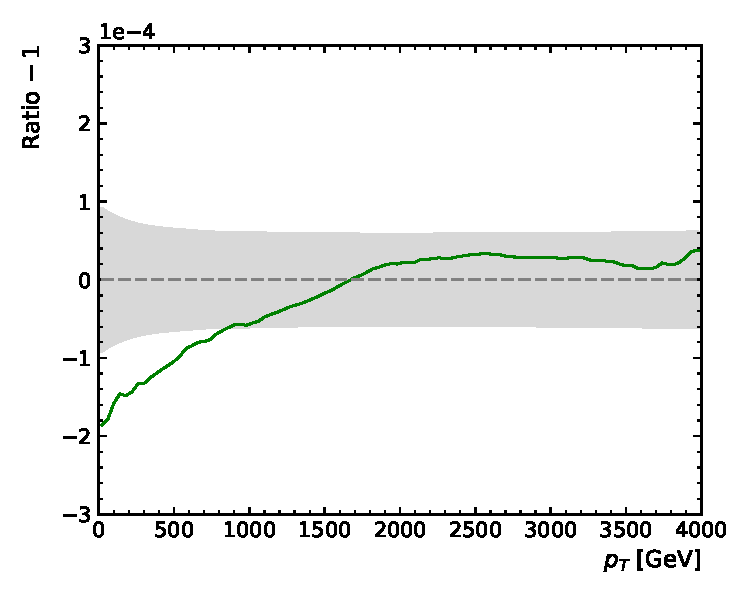
\includegraphics[width=\linewidth]{figures/sushicomparison}
  \captionof{figure}{The relative difference between the H1jet result and that of \textsc{SusHi} for the $p_T$ distribution in the MSSM. They grey band indicates the Monte Carlo error of \textsc{SusHi}.}
  \label{fig:sushicomparison}
\end{minipage}%
\hfill% 
\begin{minipage}{.485\textwidth}
  \centering
  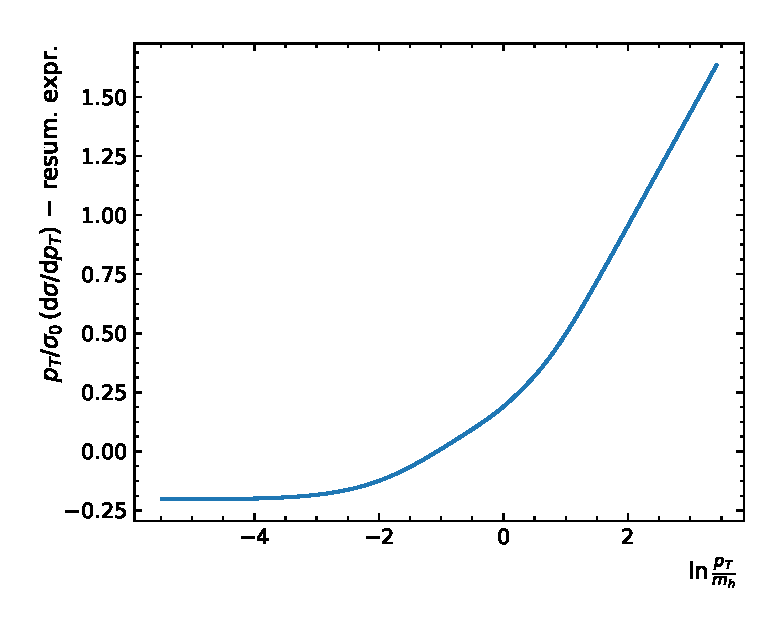
\includegraphics[width=\linewidth]{figures/sushitestlog}
  \captionof{figure}{The distribution $\frac{p_T}{\sigma_0} \left ( \frac{\mathrm{d} \sigma}{\mathrm{d} p_T} \right )$ with the first term of the $p_T$ resummation subtracted, as a function of $\ln \frac{p_T}{m_a}$. For low $p_T$ values it convergences to a constant value.}
  \label{fig:sushitestlog}
\end{minipage}
\end{figure}

\subsubsection{Relevant Options for Process: \texttt{bbH}}
If process \texttt{bbH}, i.e.\ 
\begin{equation}
	b\bar{b} \rightarrow H + \text{jet}
\end{equation}
has been selected, then the following options are relevant: 
\begin{description}[labelindent=\parindent, labelwidth =\widthof{\bfseries9999999999999999999999}, leftmargin = !] 
	\item[\texttt{--mH <value>}] Higgs mass, $m_H$ [GeV]. \\ Default: 125 GeV. 
	\item[\texttt{--vev <value>}] Higgs vacuum expectation value (VEV), $v$ [GeV]. \\ Default: 246.21846 GeV. 
	\item[\texttt{--mbmb <value>}] $\overline{\text{MS}}$ bottom quark mass, $m_b^{\overline{\text{MS}}}$ [GeV]. \\ Default: 4.18 GeV. 
\end{description}

\subsubsection{Relevant Options for Process: \texttt{Z}}
If process \texttt{Z}, i.e.\ 
\begin{equation}
	pp/p\bar{p} \rightarrow Z + \text{jet}
\end{equation}
has been selected, then the following options are relevant: 
\begin{description}[labelindent=\parindent, labelwidth =\widthof{\bfseries9999999999999999999999}, leftmargin = !] 
	\item[\texttt{--mZ <value>}] Z boson mass, $m_Z$ [GeV]. \\ Default: 91.1876 GeV.
	\item[\texttt{--GF <value>}] Fermi coupling constant, $G_F$ [GeV$^{-2}$]. \\ Default: $0.116639 \times 10^{-4}$ GeV$^{-2}$. 
	\item[\texttt{--sinwsq <value>}] Squared sine of the Weinberg angle, $\sin^2\left ( \theta_W \right )$. \\ Default: 0.231. 
\end{description}

\subsubsection{Relevant Options for Process: \texttt{user}}
In the case of process \texttt{user}, i.e.\ a custom user-specified process, any of the above physics options may be relevant if they are used in the custom amplitude code. The code will have to be inspected to determine this. The only built-in process-relevant option is: 
\begin{description}[labelindent=\parindent, labelwidth =\widthof{\bfseries9999999999999999999999}, leftmargin = !] 
	\item[\texttt{--mass <value>}] Relevant mass in the user specified process, $M$ [GeV]. Used in the scale choice and in the setup of kinematics. \\ Default: 0 GeV. 
\end{description}
Additional options may be added depending on the custom process/amplitude. See Section \ref{sec:newprocs} below for more details on the implementation of a custom process. 

\subsubsection{Output}
H1jet will print out a brief summary of the settings and parameters used, as well as the born-level cross-section $\sigma_0$, followed by the $\mathrm{d}\sigma/\mathrm{d}p_{T}$ and $\sigma(p_{T})$ for each $p_T$ bin. \\ 

The helper script \texttt{PlotH1jet.py} facilitates easy and quick plotting of the output from H1jet. The script requires Python 3 installed in order to run. Simply pipe the output from H1jet to the script: 
\begin{lstlisting}
	$ ./h1jet [options] | python PlotH1jet.py 
\end{lstlisting}
A resulting example plot with default settings in H1jet is shown in \autoref{fig:h1jetresult}. 

\begin{figure}[tbh] 
  \centering
  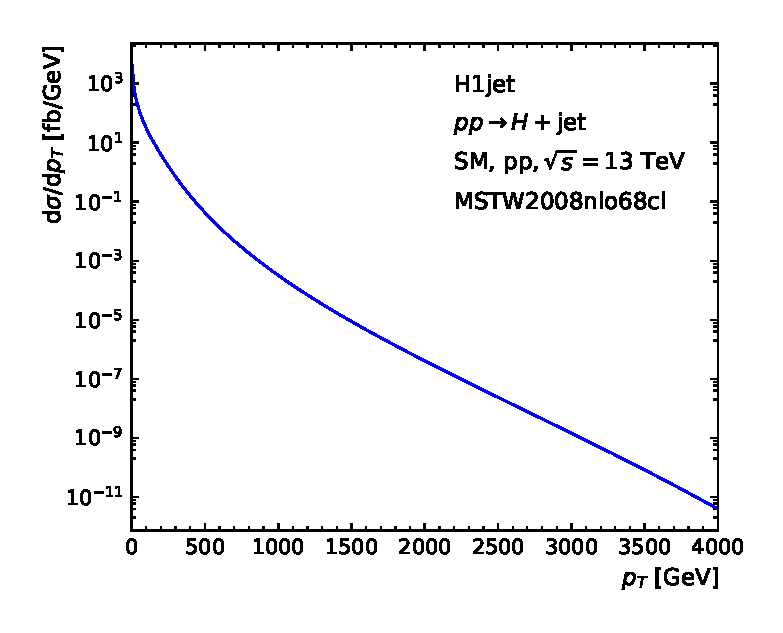
\includegraphics[width=0.6\linewidth]{figures/h1jetresult}
  \captionof{figure}{The $p_{T}$ distribution for the SM process $pp \rightarrow H + \text{jet}$ from H1jet with default settings.}
  \label{fig:h1jetresult}
\end{figure}

\section{Adding new processes to H1jet} \label{sec:newprocs} 
H1jet can be interfaced to use the squared matrix element evaluated from a custom Fortran code. The implementation may be most easily explained with a specific example. Please read this section carefully before attempting to use the interface. 

\subsection{Example: Axion-Like-Particle (ALP)}
We will present here a specific example of adding to H1jet the production of a light axion-like-particle (ALP) $a$ along with a jet, which in proton-proton collisions will occur through the following four channels, 
\begin{equation}
    \begin{split}
	g g \rightarrow g a \,, \\
	q \bar{q} \rightarrow g a \,, \\ 
	q g \rightarrow q a \,, \\ 
	\bar{q} g \rightarrow \bar{q} a \,.
	\end{split}
\end{equation}
These are all tree-level processes due to an effective ALP-gluon coupling, 
\begin{equation}
   \delta \mathcal{L}_a \supset -c_{\tilde{G}}\frac{a}{f_a} G_{\mu\nu}^{a} \tilde{G}^{a \mu\nu} \,, \label{eq:ggacoupling}
\end{equation}
as well as an effective ALP-fermion coupling, 
\begin{equation}
	\delta \mathcal{L}_a \supset i \frac{a}{f_a} \sum_{\psi = Q, L} g_{a \psi} m_{\psi} \bar{\psi} \gamma_{5} \psi \,. \label{eq:apsicoupling} 
\end{equation}
The model and the \textsc{FeynRules} \cite{bib:feynrules} model files are described and provided in ref.\ \cite{bib:alp}. We will be using \textsc{FeynCalc} \cite{bib:feyncalc} to evaluate the amplitude from the model, so we will have to convert the \textsc{FeynRules} model to a \textsc{FeynArts} \cite{bib:feynarts} model in Mathematica: 
\begin{mmaCell}{Code}
<< FeynRules` 
\end{mmaCell}
\begin{mmaCell}{Code}
LoadModel["SM.fr", "alp_linear.fr", "alp_linear_operators.fr"];  
\end{mmaCell}
\begin{mmaCell}{Code}
WriteFeynArtsOutput[LSM + LALP, CouplingRename -> False]; 
\end{mmaCell}
The resulting \textsc{FeynArts} model files are written to a new directory \texttt{ALP\_linear\_FA}, which needs to be moved to the \textsc{FeynArts/Models} directory. Note that in the \textsc{FeynArts} model, the ALP field is called \texttt{S[4]} and the gluon fields are called \texttt{V[4]}. 

In a new Mathematica session, load \textsc{FeynCalc} with \textsc{FeynArts}: 
\begin{mmaCell}{Code}
$LoadAddOns = {"FeynArts"}; 
\end{mmaCell}
\begin{mmaCell}{Code}
<< FeynCalc` 
\end{mmaCell}
The \textsc{FeynArts/Models} directory can be located with: 
\begin{mmaCell}{Code}
$FeynArtsDir
\end{mmaCell}
First patch the \texttt{ALP\_linear\_FA} model with: 
\begin{mmaCell}{Code}
FAPatch[PatchModelsOnly -> True] 
\end{mmaCell}
This ensures that the model files works with \textsc{FeynCalc}. 

Then create the tree-level $2 \rightarrow 2$ topologies and insert the fields for our process: 
\begin{mmaCell}{Code}
tops = CreateTopologies[0, 2 -> 2];
\end{mmaCell}
\begin{mmaCell}{Code}
ins = InsertFields[tops, {V[4], V[4]} -> {V[4], S[4]}, InsertionLevel -> {Classes}, Model -> "ALP_linear_FA", GenericModel -> "ALP_linear_FA"];
\end{mmaCell}
It is possible to draw the Feynman diagrams for the process as a check: 
\begin{mmaCell}{Code}
Paint[ins, ColumnsXRows -> {2, 1}, Numbering -> Simple, SheetHeader -> None, ImageSize -> {512, 256}]; 
\end{mmaCell}
We will then set up the amplitude: 
\begin{mmaCell}{Code}
feynamp = CreateFeynAmp[ins];  
\end{mmaCell}
\begin{mmaCell}{Code}
amp = FCFAConvert[feynamp, IncomingMomenta -> {k1, k2}, OutgoingMomenta -> {k3, k4}, UndoChiralSplittings -> True, ChangeDimension -> 4, TransversePolarizationVectors -> {k1, k2, k3}, List -> False, SMP -> True, Contract -> True, DropSumOver -> True] 
\end{mmaCell}
While not strictly necessary, it is recommended to enable the \texttt{SMP} option. Any additional substitutions in the amplitude can be specified with the \texttt{FinalSubstitutions} option. 

We will then set up the kinematics: 
\begin{mmaCell}{Code}
FCClearScalarProducts[]; 
\end{mmaCell}
\begin{mmaCell}{Code}
SetMandelstam[s, t, u, k1, k2, -k3, -k4, 0, 0, 0, mA]; 
\end{mmaCell}
We introduce here a parameter \texttt{mA} for the ALP mass $m_a$. 

We can then square the amplitude: 
\begin{mmaCell}{Code}
ampsquared = Simplify[
  (TrickMandelstam[#1, {s, t, u, mA^2}] & )[
    (DoPolarizationSums[#1, k2, k1, ExtraFactor -> 1/2] & )[
      (DoPolarizationSums[#1, k1, k2, ExtraFactor -> 1/2] & )[ 
        (DoPolarizationSums[#1, k3, 0] & )[ 
          (SUNSimplify[#1, Explicit -> True, SUNNToCACF -> False] & )[
            FeynAmpDenominatorExplicit[(1 / (SUNN^2 - 1)^2) * (amp * ComplexConjugate[amp])]]]]]]] /. SUNN -> 3 
\end{mmaCell}
Setting the \texttt{SUNNToCACF} option in \texttt{SUNSimplify[]} to \texttt{False} is not necessary, nor is it necessary to fix \texttt{SUNN} to $3$. This can be handled by the dressing script and H1jet. 

Finally, we will write the amplitude as Fortran code to a file: 
\begin{mmaCell}{Code}
Write2["ALP_amp.f90", gg = ampsquared, FormatType -> FortranForm, FortranFormatDoublePrecision -> False] 
\end{mmaCell}
Note here that we specify the gluon-gluon channel with the \texttt{gg = ampsquared} input to the function. This is required for the subsequent dressing script to work properly. It is important to specify the $2$-particle initial state by using combinations of \texttt{g}, \texttt{u}, \texttt{d}, \texttt{c}, \texttt{s}, \texttt{b}, \texttt{ubar}, \texttt{dbar}, \texttt{cbar}, \texttt{sbar}, and \texttt{bbar}. One can also use \texttt{q} and \texttt{qbar} for all the light quarks and antiquarks respectively, i.e.\ $u$, $d$, $c$, and $s$. For example, \texttt{bbbar} will be the $b\bar{b}$ channel. \\ 

The generated Fortran code \texttt{ALP\_amp.f90} will have to be dressed by the Python helper script \texttt{DressUserAmpCode.py}: 
\begin{lstlisting}
	$ python DressUserAmpCode.py ALP_amp.f90 
\end{lstlisting}
This will produce a dressed Fortran code file by default called \texttt{user\_interface.f90}. 

The helper script has a help message which can be called with \texttt{-h} or \texttt{--help}. The name of the output file can be specified with the \texttt{-o} option. Multiple input Fortran files can be provided to the helper script. The full usage is: 
\begin{lstlisting}
	$ python DressFeynCalcCode.py [-h] [-o [OUTFILE]] inputfile [inputfile ...] 
\end{lstlisting}
The provided input Fortran code files does not necessarily have to be generated with \textsc{FeynCalc}. They can be generated by any other program or even be written by hand. \\ 

To use the new dressed custom Fortran code with H1jet, it is necessary to compile H1jet with the custom Fortran code: 
\begin{lstlisting}
	$ make USERPATH=<path/to/code> 
\end{lstlisting}
Running \texttt{./h1jet --help} we see that three new additional options have been added: 
\begin{description}[labelindent=\parindent, labelwidth =\widthof{\bfseries9999999999999999999999}, leftmargin = !] 
	\item[\texttt{--c\_CGtil <value>}] The Wilson coefficient $c_{\tilde{G}}$ in \autoref{eq:ggacoupling}. 
	\item[\texttt{--c\_mA <value>}] The ALP mass, $m_a$. 
	\item[\texttt{--c\_fa <value>}] The ALP suppression scale $f_a$ in \autoref{eq:ggacoupling}. 
\end{description}
The leading \texttt{c\_} in the name stands for ``custom'' and is automatically added in order to avoid naming issues in the code. \\ 

The result from the ALP implementation in H1jet has been compared to the result for the same \textsc{FeynRules} model used with \textsc{MadGraph5\_aMC@NLO} \cite{bib:mg5}. The comparison is shown in \autoref{fig:alpbenchmark} and \ref{fig:alpratio}, where we see nice agreement. 

\begin{figure}[tbh] 
\centering
\begin{minipage}{.485\textwidth}
  \centering
  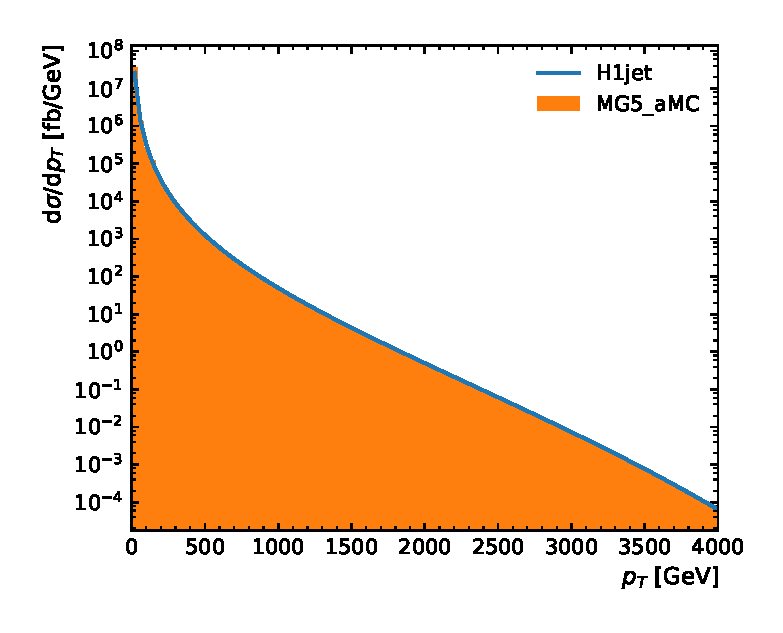
\includegraphics[width=\linewidth]{figures/alpresult}
  \captionof{figure}{The $p_{T}$ distribution for the process $gg \rightarrow ga$ from H1jet with the amplitude from \textsc{FeynCalc} (blue line) compared to \textsc{MadGraph5\_aMC@NLO} (orange bins).}
  \label{fig:alpbenchmark}
\end{minipage}%
\hfill% 
\begin{minipage}{.485\textwidth}
  \centering
  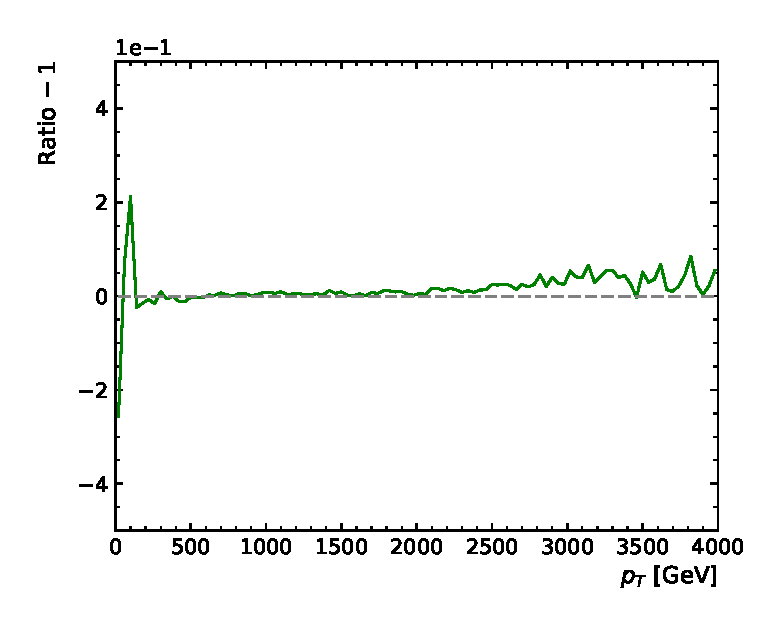
\includegraphics[width=\linewidth]{figures/alpratio}
  \captionof{figure}{The ratio between the result from H1jet with the amplitude from \textsc{FeynCalc} and the result from \textsc{MadGraph5\_aMC@NLO}.}
  \label{fig:alpratio}
\end{minipage}
\end{figure}

The low $p_T$ behaviour in \autoref{fig:alpratio} is due to possible numerical instability. The H1jet result can be further checked in the $p_{T} \rightarrow 0$ limit, by comparing it to the resummation expression, 
\begin{equation}
	\frac{\mathrm{d} \sigma}{\mathrm{d} p_T} \xrightarrow{p_T \rightarrow 0} \sigma_0 \left [ 4 C_A \frac{\alpha_s}{\pi} \frac{1}{p_T} \ln\left ( \frac{m_a}{p_T} \right ) + \mathcal{O} ( \alpha_s^2 ) \right ] \,, \label{eq:resum}
\end{equation}
where $\sigma_0$ is the total born-level cross-section for $gg \rightarrow a$. In \autoref{fig:alpresum}, we show $\frac{p_T}{\sigma_0} \left ( \frac{\mathrm{d} \sigma}{\mathrm{d} p_T} \right )$ with the first term of \autoref{eq:resum} subtracted, as a function of $\ln \frac{p_T}{m_a}$. For $p_T \rightarrow 0$ this goes nicely towards a constant as expected. 

\begin{figure}[tbh] 
  \centering
  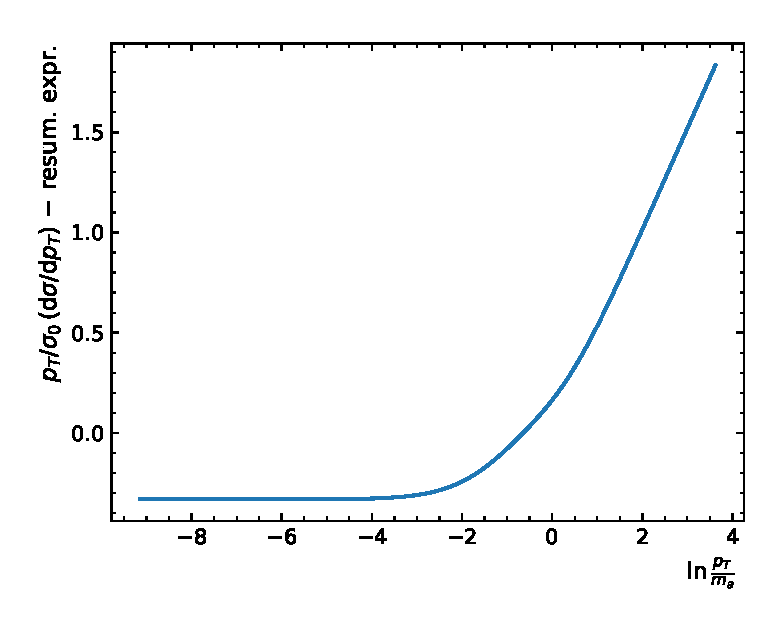
\includegraphics[width=0.6\linewidth]{figures/alpresum}
  \captionof{figure}{The distribution $\frac{p_T}{\sigma_0} \left ( \frac{\mathrm{d} \sigma}{\mathrm{d} p_T} \right )$ with the first term of the $p_T$ resummation subtracted, as a function of $\ln \frac{p_T}{m_a}$.}
  \label{fig:alpresum}
\end{figure}

\ifstandalone
\begin{thebibliography}{1}
   \bibitem{bib:h1jet} H1jet can be downloaded from: \\ \href{https://h1jet.hepforge.com}{https://h1jet.hepforge.com}
   \bibitem{bib:lhapdf} A.\ Buckley, J.\ Ferrando, S.\ Lloyd, K.\ Nordstrom, B.\ Page, M.\ Ruefenacht, M.\ Schoenherr, and G.\ Watt, \textit{LHAPDF6: parton density access in the LHC precision era}, Eur.\ Phys.\ J.\ \textbf{C75} (2015) 3, 132, [\href{https://arxiv.org/abs/1412.7420}{arXiv:1412.7420}]. 
   \bibitem{bib:hoppet} G.\ P.\ Salam and J.\ Rojo, \textit{A Higher Order Perturbative Parton Evolution Toolkit (HOPPET)}, Comput.\ Phys.\ Commun.\ \textbf{180} (2009) 120-156, [\href{https://arxiv.org/abs/0804.3755}{arXiv:0804.3755}]. 
   \bibitem{bib:chaplin} S.\ Buehler and C.\ Duhr, \textit{CHAPLIN - Complex Harmonic Polylogarithms in Fortran}, Comput.\ Phys.\ Commun.\ \textbf{185} (2014) 2703, [\href{https://arxiv.org/abs/1106.5739}{arXiv:1106.5739}]. 
   \bibitem{bib:mssm1} J.\ F.\ Gunion, H.\ E.\ Haber, \textit{The CP-conserving two-Higgs-doublet model: the approach to the decoupling limit}, Phys.\ Rev.\ D \textbf{67}, 075019 (2003), [\href{https://arxiv.org/abs/hep-ph/0207010}{arXiv:hep-ph/0207010}]. 
   \bibitem{bib:mssm2} A.\ Banfi, A.\ Bond, A.\ Martin, and V.\ Sanz, \textit{Digging for Top Squarks from Higgs data: from signal strengths to differential distributions}, J. High Energ. Phys. \textbf{2018}, 171 (2018), [\href{https://arxiv.org/abs/1806.05598}{arXiv:1806.05598}]. 
   \bibitem{bib:sushi} R.\ V.\ Harlander, S.\ Liebler, and H.\ Mantler, \textit{SusHi: A program for the calculation of Higgs production in gluon fusion and bottom-quark annihilation in the Standard Model and the MSSM}, Comput.\ Phys.\ Commun.\ \textbf{184} (2013) 1605–1617, \textbf{2018}, 171 (2018), [\href{https://arxiv.org/abs/1212.3249}{arXiv:1212.3249}]; R.\ V.\ Harlander, S.\ Liebler, and H.\ Mantler, \textit{SusHi Bento: Beyond NNLO and the heavy-top limit}, Comput.\ Phys.\ Commun.\ \textbf{212} (2017) 239–257, [\href{https://arxiv.org/abs/1605.03190}{arXiv:1605.03190}]. \\ \href{https://sushi.hepforge.org}{https://sushi.hepforge.org} 
   \bibitem{bib:feynrules} A.\ Alloul, N.\ D.\ Christensen, C.\ Degrande, C.\ Duhr, and B.\ Fuks, \textit{FeynRules 2.0 - A complete toolbox for tree-level phenomenology}, Comput.\ Phys.\ Commun.\ \textbf{185} (2014) 2250-2300, [\href{https://arxiv.org/abs/1310.1921}{arXiv:1310.1921}]. \\ \href{https://feynrules.irmp.ucl.ac.be}{https://feynrules.irmp.ucl.ac.be} 
   \bibitem{bib:alp} I.\ Brivio, M.\ B.\ Gavela, L.\ Merlo, K.\ Mimasu, J.\ M.\ No, R.\ del Rey, and V.\ Sanz, \textit{ALPs Effective Field Theory and Collider Signatures}, Eur.\ Phys.\ J.\ \textbf{C77} (2017) 572, [\href{https://arxiv.org/abs/1701.05379}{arXiv:1701.05379}]. The \textsc{FeynRules} model file is available here: \href{https://feynrules.irmp.ucl.ac.be/wiki/ALPsEFT}{https://feynrules.irmp.ucl.ac.be/wiki/ALPsEFT}. 
   \bibitem{bib:feyncalc} V.\ Shtabovenko, R.\ Mertig, and F.\ Orellana, \textit{FeynCalc 9.3: New features and improvements}, [\href{https://arxiv.org/abs/2001.04407}{arXiv:2001.04407}]; V.\ Shtabovenko, R.\ Mertig, and F.\ Orellana, \textit{New Developments in FeynCalc 9.0}, Comput.\ Phys.\ Commun.\ \textbf{64} (1991) 345-359, [\href{https://arxiv.org/abs/1601.01167}{arXiv:1601.01167}]; R.\ Mertig, M.\ Böhm, and A.\ Denner, \textit{Feyn Calc - Computer-algebraic calculation of Feynman amplitudes}, Comput.\ Phys.\ Commun.\ \textbf{64} (1991) 345-359. \\ \href{https://feyncalc.github.io}{https://feyncalc.github.io} 
   \bibitem{bib:feynarts} T.\ Hahn, \textit{Generating Feynman diagrams and amplitudes with FeynArts 3}, Comput.\ Phys.\ Commun.\ \textbf{140} (2001) 418-431, [\href{https://arxiv.org/abs/hep-ph/0012260}{arXiv:hep-ph/0012260}]. \\ \href{http://www.feynarts.de}{http://www.feynarts.de} 
   \bibitem{bib:mg5} J.\ Alwall, R.\ Frederix, S.\ Frixione, V.\ Hirschi, F.\ Maltoni, O.\ Mattelaer, H.-S.\ Shao, T.\ Stelzer, P.\ Torrielli, and M.\ Zaro, \textit{The automated computation of tree-level and next-to-leading order differential cross sections, and their matching to parton shower simulations}, [\href{https://arxiv.org/abs/1405.0301}{arXiv:1405.0301}]. \\ \href{https://launchpad.net/mg5amcnlo}{https://launchpad.net/mg5amcnlo} 
\end{thebibliography}

\end{document}
\fi


\section{Conclusions}
\label{sec:the-end}

\paragraph{Acknowledgements.}

\appendix

\section{Implementation of scalar integrals}
\label{sec:scalar-integrals}

This appendix contains the details of how H1jet computes one-loop
scalar integrals that are relevant for Higgs production. These
integrals depend on one internal mass, which we denot by $m$, and are
functions of Lorentz invariant quantities, typically Mandelstam
invariants.

These integrals contains logarithms and dilogarithms of complex
arguments, which require appropriate analytic continuations. We have
decided to use CHAPLIN, and recast all relevant trascendental
functions into harmonic polylogarithms $H(\vec a;z)$, with
$\vec a=(a_1,\dots,a_n)$. For real values of the argument, CHAPLIN
uses the $+i\varepsilon$ prescription, i.e.\ $H(\vec a;z)$ with $z$
real is interpreted as $H(\vec a;z+i\varepsilon)$. Therefore, we need
to make sure that the imaginary part of the argument of scalar
integrals is consistent with CHAPLIN.

The relevant one-loop integrals we need to deal with are of  three kinds, 
bubbles, triangles and boxes.

\paragraph{Bubbles.} The bubble integral is defined as
\begin{equation}
  \label{eq:bubble}
  B_0(s)=2 -\sqrt{1-\frac{4(m^2-i\varepsilon)}{s}}\ln\left[-\frac{z}{1-z}\right]\,,
\end{equation}
where 
\begin{equation}
  \label{eq:z}
  z=\frac{1}{2}\left(1+\sqrt{1-\frac{4(m^2-i\varepsilon)}{s}}\right)\,.
\end{equation}
The argument of the logarithm in eq.~\eqref{eq:bubble} has a different
from according to the value of $s$:
\begin{equation}
  \label{eq:z-omz}
  -\frac{z}{1-z} = \left\{
    \begin{split}
      &-\frac{1+\sqrt{1+\frac{4m^2}{|s|}}}{1-\sqrt{1+\frac{4m^2}{|s|}}}\,,\qquad \qquad s<0\,,\\
        & -\frac{1+i\sqrt{\frac{4m^2}{s}-1}}{1-i\sqrt{\frac{4m^2}{s}-1}}\,,\qquad \quad\>\> 0<s<4m^2\,,\\
        &
        -\frac{1-\sqrt{1-\frac{4m^2}{s}}}{1-\sqrt{1-\frac{4m^2}{s}}}-i\varepsilon\,,\qquad
        s>4m^2
    \end{split}
\right.
\end{equation}
Note that the only case in which one needs a small imaginary part is
the case $s>4m^2$. This imaginary part has the opposite convention as
in CHAPLIN. As a solution, we invert the argument of the logarithm and
use the identity $\ln(1/z)=-\ln(z)$. Practically, analytically
continuing the square root, we use
\begin{equation}
  \label{eq:z-implemented}
  z = \left\{\begin{split}
      \frac{1}{2}\left(1+i\sqrt{\frac{4m^2}{s}-1}\right)\,,& \qquad s< 4m^2\\
      \frac{1}{2}\left(1+\sqrt{1-\frac{4m^2}{s}}\right)\,,& \qquad s> 4m^2
    \end{split}
    \right.
  \end{equation}
and implement the bubble as follows:
\begin{equation}
  \label{eq:bubble-implemented}
  B_0(s)=
    2 +(2 z-1) \,H\left(0,\frac{z}{z-1}\right) \,.
\end{equation}

 
\paragraph{Triangles.} The triangle integral $C_0(s)$ is defined as
\begin{equation}
  \label{eq:triangle}
  C_0(s) = \frac{1}{2s}\ln^2\left[-\frac{z}{1-z}\right]\,,
\end{equation}
where $z$ is given in eq.~\eqref{eq:z}. Again, for $s>4m^2$, the argument of the logarithm has the opposite convention as CHAPLIN. Therefore, we invert again the argument of the logarithm, and using the definition of $z$ in eq.~\eqref{eq:z-implemented}, we implement the triangle as follows:
\begin{equation}
  \label{eq:triangle-HPL}
  s\,C_0(s) = H\left(0,0;\frac{z-1}{z}\right)\,.
\end{equation}

\paragraph{Boxes.}

\begin{thebibliography}{1}
   \bibitem{bib:h1jet} H1jet can be downloaded from: \\ \href{https://h1jet.hepforge.com}{https://h1jet.hepforge.com}
   \bibitem{bib:lhapdf} A.\ Buckley, J.\ Ferrando, S.\ Lloyd, K.\ Nordstrom, B.\ Page, M.\ Ruefenacht, M.\ Schoenherr, and G.\ Watt, \textit{LHAPDF6: parton density access in the LHC precision era}, Eur.\ Phys.\ J.\ \textbf{C75} (2015) 3, 132, [\href{https://arxiv.org/abs/1412.7420}{arXiv:1412.7420}]. 
   \bibitem{bib:hoppet} G.\ P.\ Salam and J.\ Rojo, \textit{A Higher Order Perturbative Parton Evolution Toolkit (HOPPET)}, Comput.\ Phys.\ Commun.\ \textbf{180} (2009) 120-156, [\href{https://arxiv.org/abs/0804.3755}{arXiv:0804.3755}]. 
   \bibitem{bib:chaplin} S.\ Buehler and C.\ Duhr, \textit{CHAPLIN - Complex Harmonic Polylogarithms in Fortran}, Comput.\ Phys.\ Commun.\ \textbf{185} (2014) 2703, [\href{https://arxiv.org/abs/1106.5739}{arXiv:1106.5739}]. 
   \bibitem{bib:alp} I.\ Brivio, M.\ B.\ Gavela, L.\ Merlo, K.\ Mimasu, J.\ M.\ No, R.\ del Rey, and V.\ Sanz, \textit{ALPs Effective Field Theory and Collider Signatures}, Eur.\ Phys.\ J.\ \textbf{C77} (2017) 572, [\href{https://arxiv.org/abs/1701.05379}{arXiv:1701.05379}]. The \textsc{FeynRules} model file is available here: \href{https://feynrules.irmp.ucl.ac.be/wiki/ALPsEFT}{https://feynrules.irmp.ucl.ac.be/wiki/ALPsEFT}. 
\end{thebibliography}

\end{document}
